\documentclass[a4paper,ngerman,12pt]{scrartcl}

\usepackage[utf8]{inputenc}
%\usepackage[ansinew]{inputenc}

\usepackage[ngerman]{babel}

\usepackage{amsmath,amsthm,amssymb,stmaryrd,color,graphicx}
\usepackage{setspace}
\usepackage{bussproofs}
\usepackage{array}
\usepackage{comment}
\usepackage{wrapfig}

\usepackage{enumitem}

\usepackage{units}

\usepackage[protrusion=true,expansion=true]{microtype}

\usepackage{lmodern}

\usepackage{hyperref}
\usepackage{cleveref}

\newcommand{\RR}{\mathbb{R}}
\newcommand{\CC}{\mathbb{C}}
\newcommand{\ZZ}{\mathbb{Z}}
\newcommand{\NN}{\mathbb{N}}
\newcommand{\QQ}{\mathbb{Q}}

\setlength\parskip{\medskipamount}
\setlength\parindent{0pt}

\theoremstyle{definition}
\newtheorem{defn}{Definition}[]
\newtheorem{axiom}[defn]{Axiom}
\newtheorem{bsp}[defn]{Beispiel}

\theoremstyle{plain}
\newtheorem{prop}[defn]{Proposition}
\newtheorem{motto}[defn]{Motto}
\newtheorem{wunder}[defn]{Wunder}
\newtheorem{ueberlegung}[defn]{Überlegung}
\newtheorem{lemma}[defn]{Lemma}
\newtheorem{kor}[defn]{Korollar}
\newtheorem{hilfsaussage}[defn]{Hilfsaussage}
\newtheorem{satz}[defn]{Satz}
\newtheorem{frage}[defn]{Frage}

\theoremstyle{remark}
\newtheorem{bem}[defn]{Bemerkung}
\newtheorem{aufg}[defn]{Aufgabe}

\newtheorem*{antwort}{Antwort}

\newlength{\aufgabenskip}
\setlength{\aufgabenskip}{1.4em}
\newcounter{aufgabennummer}
\newenvironment{aufgabe}[1]{
	\addtocounter{aufgabennummer}{1}
	\textbf{Aufgabe \theaufgabennummer.} \emph{#1} \par
}{\vspace{\aufgabenskip}}

\clubpenalty=10000
\widowpenalty=10000
\displaywidowpenalty=10000

\setlength\unitlength{1cm}

\usepackage{tikz}

\RequirePackage{geometry}
\geometry{textwidth=16.0cm,textheight=24.5cm,footskip=1.5cm}

\begin{document}
	
\begin{picture}(0,0)
\put(0,-0.5){%
	
\includegraphics[scale=0.1]{logo-ifm}
}
\put(14.0,-3.5){%
	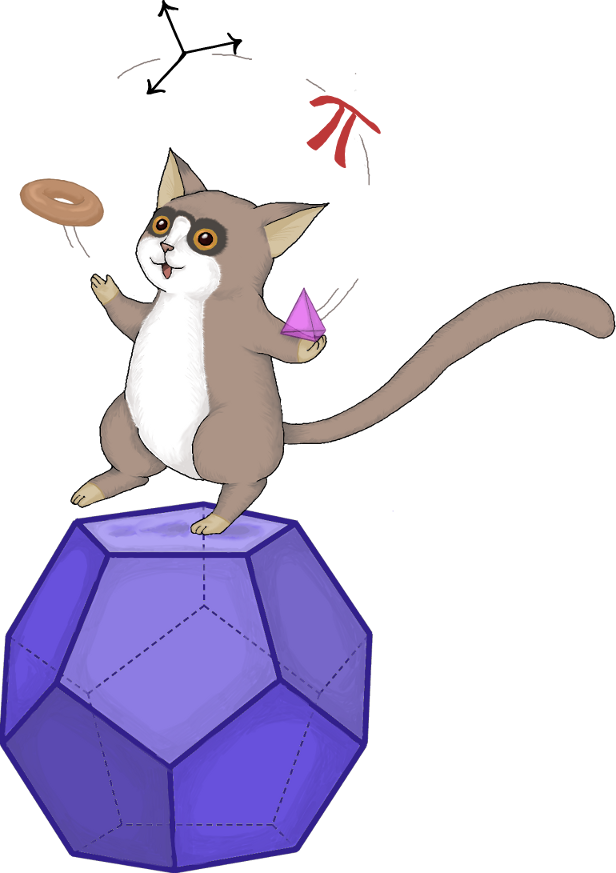
\includegraphics[scale=0.17]{cover}
}
\end{picture} 
	
\vspace{6em}

\begin{center}\Large{Fünfter Korrespondenzbrief}\end{center}

\section*{Unmöglichkeitsbeweise über Invarianten}

\begin{wrapfigure}{r}{0.28\textwidth}\vspace{-50pt}
	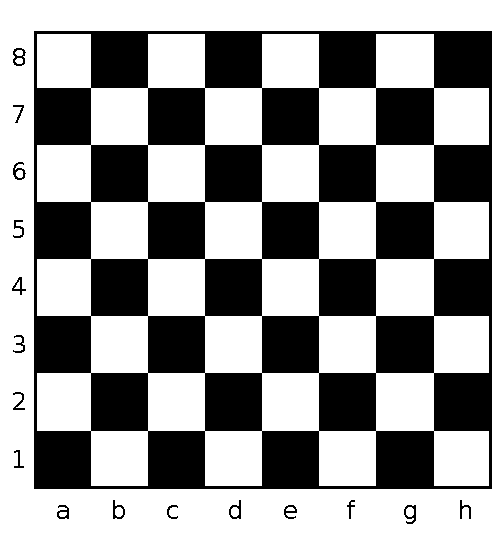
\includegraphics[width=.28\textwidth]{Bilder/Schachbrett.pdf}
\vspace{-50pt}\end{wrapfigure}

Vor uns befindet sich ein leeres Schachbrett und ein großer Haufen Dominosteine. Ein Dominostein ist genauso groß wie zwei Felder des Schachbretts. Wenn du magst, kannst du dir das Schachbrett, die Dominosteine und ein paar Tetris-Steine (die übrigens auch Tetrominos genannt werden), die wir später noch brauchen werden, auf der letzten Seite dieses Briefes ausschneiden und selbst mitknobeln.

\begin{frage}
	Ist es möglich, das Schachbrett mit Dominosteinen so zu belegen, dass jedes Feld bedeckts ist, keine zwei Dominosteine übereinander liegen und kein Stein über den Rand hinausragt? 
\end{frage}

\begin{antwort}
	Ja. Eine Möglichkeit (von vielen) in jede Zeile vier Dominosteine nebeneinander zu legen.
\end{antwort}

Wir sägen nun aus dem Schachbrett die rechte untere Ecke, das Feld \emph{h1}, heraus.

\begin{frage}
	Ist es immer noch möglich, das Schachbrett wie beschrieben mit Dominosteinen zu belegen? Probiere es einmal aus!
\end{frage}

\begin{antwort}
	Du wirst vermutlich schnell feststellen, dass es diesmal nicht zu funktionieren scheint - und das hat einen ganz einfachen Grund: Das Schachbrett ohne rechte untere Ecke hat 63 Felder. Jeder Dominostein belegt genau zwei Felder. Wenn eine Überdeckung möglich wäre, so hätte das Schachbrett ohne rechte untere Ecke somit eine gerade Anzahl von Feldern. Also kann es keine Überdeckung geben.
\end{antwort}

Während wir die erste Frage einfach positiv (bejahend) beantworten konnten, indem wir eine Überdeckung mit Dominosteinen angegeben haben, fällt uns die negative (verneinende) Antwort etwas schwerer: Wir mussten nämlich einen Grund finden, warum es eine solche Überdeckung nicht geben kann. Es reicht nicht aus, zu sagen, man habe keine Lösung gefunden. Es könnte ja immer noch sein, dass man sich nur ungeschickt angestellt hat und deshalb keine Lösung gefunden hat.

\begin{wrapfigure}{r}{0.14\textwidth}\vspace{-20pt}
	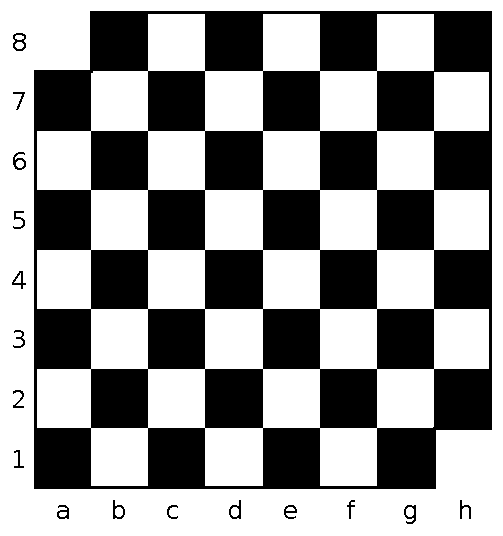
\includegraphics[width=.14\textwidth]{Bilder/Schachbrett2.pdf}
	\vspace{-40pt}\end{wrapfigure}

Wir sägen nun aus dem Schachbrett auch die linke obere Ecke, das Feld \emph{h8}, heraus.

\begin{frage}
	Wie immer: Gibt es nun eine Überdeckung des Schachbretts mit Dominosteinen?
\end{frage}

Das Schachbrett ohne die beiden Ecken hat nun wieder eine gerade Anzahl von Feldern, nämlich 62. Prinzipiell könnte also eine Überdeckung möglich sein. Wenn du aber versuchst, eine zu finden, wirst du feststellen, dass - egal wie du dich anstellst - immer zwei Felder übrig bleiben. Es liegt daher die Vermutung nahe, dass es erneut unmöglich ist, eine Überdeckung zu finden. Um wirklich sicher sein zu können, müssen wir aber einen Beweis dafür finden: 

\begin{antwort}
	Nein. Wenn man einen Dominostein auf das Brett legt, so bedeckt er, egal wie er liegt, ein weißes und ein schwarzes Feld. Die beiden Felder, die wir abgesägt haben, waren beides weiße Felder. Damit hat das um zwei Ecken verkleinerte Brett noch 30 weiße und 32 schwarze Felder. Jedes Mal, wenn wir einen Stein setzen, nimmt die Zahl der noch offenen weißen und die Zahl der noch offenen schwarzen Felder um je 1 ab. Nach drei gelegten Dominosteinen haben wir beispielsweise noch $30-3=27$ offene weiße und $32-3=29$ offene schwarze Felder. Zu jedem Zeitpunkt gibt es genau zwei schwarze unbedeckte Felder mehr als weiße unbedeckte Felder. Wenn alle weißen Felder bedeckt sind, gibt es also noch zwei schwarze offene Felder. Diese können aber nicht nebeneinander liegen, deshalb können sie nicht mit einem Domino überdeckt werden.
\end{antwort}

Wären nicht zwei diagonal gegenüberliegende, sondern zwei Ecken, die an einer Seite liegen, herausgesägt worden, so wäre die Aufgabe lösbar gewesen (findest du einen Weg wie?).

\section{Tetrominoparkett}

Als nächstes wollen wir statt den Dominos, die zwei Felder überdecken, Steine betrachten, die vier Felder groß sind - die Tetrominos:

\begin{center}
	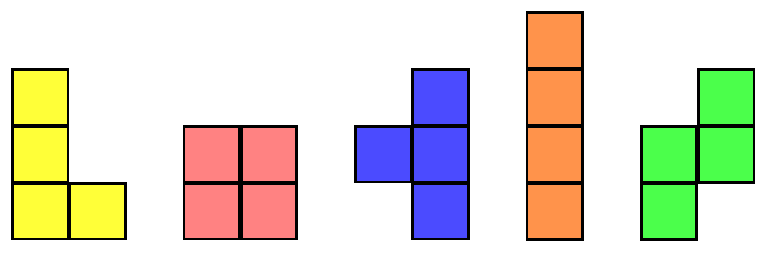
\includegraphics[width=.6\textwidth]{Bilder/Tetrominos.pdf}
\end{center}

\begin{aufgabe}{}
	Als erstes betrachten wir den roten Tetrominostein (das 2x2-Quadrat). Welches der folgenden Schachbretter kannst du nur mit solchen Steinen überdecken? 
	
	\begin{center}
		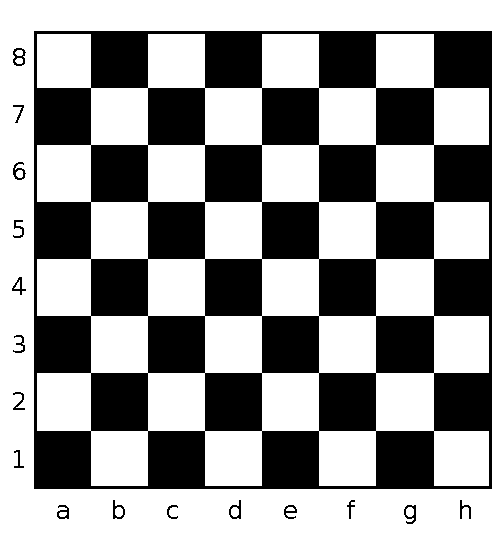
\includegraphics[width=.2\textwidth]{Bilder/Schachbrett.pdf}
		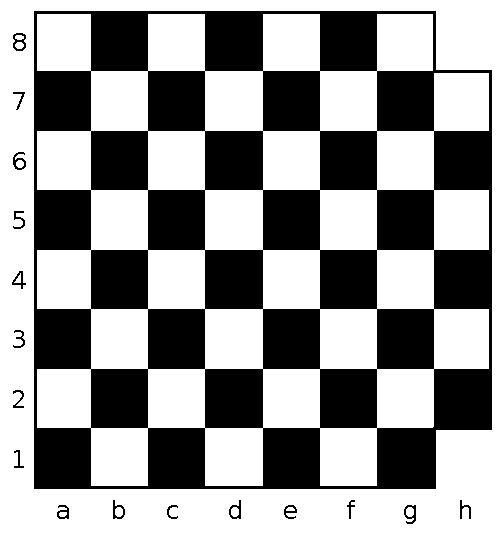
\includegraphics[width=.2\textwidth]{Bilder/Schachbrett3.pdf}
		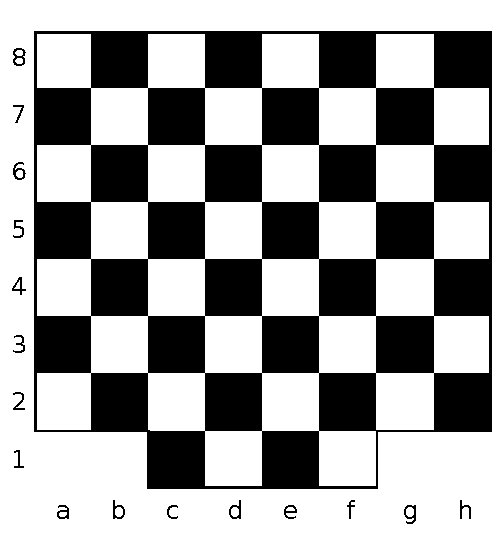
\includegraphics[width=.2\textwidth]{Bilder/Schachbrett4.pdf}
		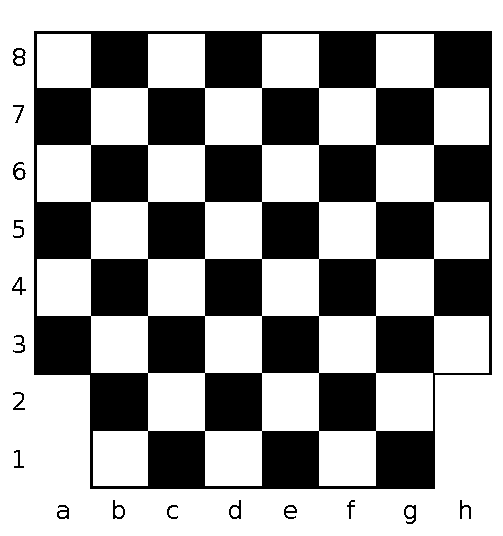
\includegraphics[width=.2\textwidth]{Bilder/Schachbrett5.pdf}
	\end{center}
	
	Wenn es möglich ist, beschreibe eine solche Überdeckung (oder zeichne sie). Wenn keine Überdeckung möglich ist, versuche einen Beweis dafür zu finden (wie bei den Fragen 2 und 3).
	
	\emph{Hinweis:} Um einen Unmöglichkeitsbeweis der Form von Frage 3 zu führen, genügt diesmal ein normales zweifarbiges Schachbrett nicht. Stattdessen ist hier ein - in passender Weise - in vier Farben gefärbtes \glqq Schachbrett\grqq{} hilfreich (schließlich haben wir ja jetzt auch Steine, die vier Felder überdecken). Auf der letzten Seite dieses Briefes findest du zwei Vorschläge für eine entsprechende Färbung.
\end{aufgabe}

\begin{aufgabe}{}
	Nun verwenden wir den orangen Tetrominostein (das lange 4x1-Rechteck). Welches der Schachbretter aus Aufgabe 1 kannst du nur mit solchen Steinen überdecken? 
	
	Wenn es möglich ist, beschreibe eine solche Überdeckung (oder zeichne sie). Wenn keine Überdeckung möglich ist, versuche einen Beweis dafür zu finden (wie bei den Fragen 2 und 3).
	
	\emph{Hinweis:} Auch hier ist unter Umständen eines der vierfarbigen \glqq Schachbretter\grqq{} hilfreich.
\end{aufgabe}

Um die Sache etwas bunter zu machen, wollen wir nun alle fünf Tetrominos auf einmal verwenden - jeden aber nur genau einmal. Offenbar ist es nicht möglich damit das gesamte Schachbrett zu überdecken (warum?). Daher werden wir uns damit begnügen einen Teil des Brettes zu überdecken:

\begin{frage}
	Ist es möglich, aus den obigen fünf Figuren ein Rechteck zu legen? Dabei dürfen sich die Figuren nicht überlappen, aber beliebig oft gedreht oder gespiegelt werden.
\end{frage}

Bevor du weiter liest, probiere es doch selbst einmal aus! Überlege dir zunächst welche Größe ein Rechteck überhaupt haben darf, damit es mit Hilfe der fünf Tetrominosteine überdeckt werden kann: Kann es ein 2x10-Rechteck sein, ein 3x5 Rechteck, ein 4x5-Rechteck, ...? Wenn du eine passende Größe gefunden hast, versuche eine entsprechende Überdeckung zu finden - d.h. die fünf Steine so zusammen zu legen, dass sie ein Rechteck ergeben. Was stellst du dabei fest?

\begin{antwort}
	Zunächst einmal stellen wir fest, dass die fünf Figuren insgesamt $5 \cdot 4 = 20$ Felder belegen. Also muss das Rechteck, falls es existiert, entweder $1$ Feld breit und $20$ Felder lang oder $2$ Felder breit und $10$ Felder lang oder $4$ Felder breit und $5$ Felder lang sein. Offensichtlich scheidet die erste Möglichkeit aus. Man kann sich auch recht schnell überlegen, dass auch die zweite Möglichkeit nicht in Frage kommt (Tipp: platziere das orange Teil zuerst). Somit bleibt nur das $5 \times 4$-Rechtecks als Möglichkeit übrig. Wenn wir aber versuchen, solch ein Rechteck mit obigen Figuren zu belegen, scheitern wir immer wieder. Das hat auch einen Grund:
	
	\begin{center}
		\emph{Es ist nicht möglich, aus den Tetris-Figuren ein Rechteck zu legen.}
	\end{center}
	
	Um das zu beweisen legen wir die Figuren (irgendwie) auf ein Schachbrett:
	
	\begin{center}
		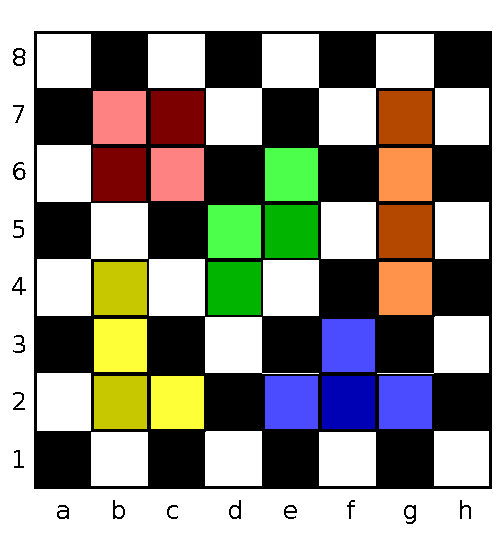
\includegraphics[width=.4\textwidth]{Bilder/Schachbrett-mit-Tetrominos.pdf}
	\end{center}	
	
	Nun fällt etwas auf: Alle Figuren bis auf die blaue belegen je zwei weiße und zwei schwarze Felder (egal, wie man sie hinlegt). Die blaue Figur, jedoch, belegt drei weiße Felder und nur ein schwarzes Feld (oder umgekehrt). Damit belegen die Figuren zusammengenommen ungleich viele weiße wie schwarze Felder, egal wie man sie anordnet. Damit kann man insbesondere kein $4 \times 5$-Rechteck mit ihnen legen, denn jedes $4 \times 5$-Rechteck auf einem Schachfeld hat gleich viele weiße und schwarze Felder.
\end{antwort}

\begin{aufgabe}{Dreieckstetrominos}
	Als kleine Abwandlung der obigen Aufgabe wollen wir nun aus Dreiecken zusammengesetzte \glqq Tetrominos\grqq{} betrachten:
	\begin{center}
		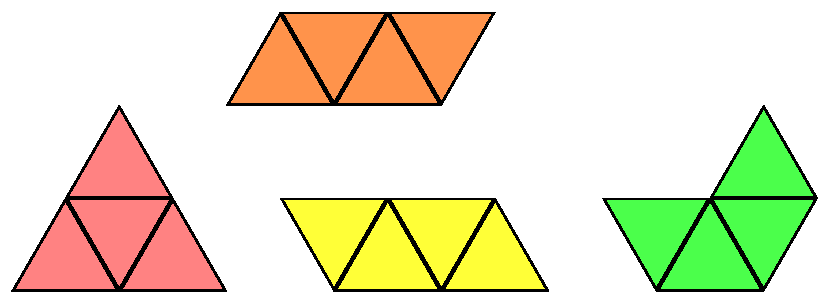
\includegraphics[width=.4\textwidth]{Bilder/Dreieckstetrominos.pdf}
	\end{center}
	Die Frage ist nun: Lassen sich diese vier Steine so zusammensetzen, dass sie ein (gleichseitiges) Dreieck ergeben? (Drehen und Spiegeln der Steine ist selbstverständlich wieder erlaubt)
	
	\emph{Hinweis:} Evtl. ist es wieder hilfreich, die Steine auf eine Art \glqq Schachbrett\grqq{} zu legen - nur benötigst du diesmal natürlich eines aus Dreiecken. Du findest ein solches auf der letzten Seite des Briefes.
\end{aufgabe}


\section{Teilbarkeitsinvarianten}

Auf einer Insel leben 345 gelbe, 346 grüne und 347 blaue Chamäleons. Wann immer sich zwei Chamäleons gleicher Farbe begegnen, passiert nichts. Wenn sich aber zwei Chamäleons unterschiedlicher Farbe begegnen, so nehmen beide die dritte Farbe an. Beispielsweise hätten wir nach einem Treffen eines gelben und einer grünen Chamäleons nur noch 344 gelbe, 345 grüne, aber dafür 349 blaue Chamäleons. Frage: Ist es möglich, dass zu einem Zeitpunkt genau gleich viele Chamäleons jeder Farbe auf der Insel leben?

\emph{Hinweis:} Um die Situation etwas übersichtlicher zu machen, kannst du das ganze erstmal auch nur mit 1 gelben, 2 grünen und 3 blauen Chamäleons durchspielen. Das Ergebnis wird das gleiche sein.

% Bildquelle: http://commons.wikimedia.org/wiki/File:Cham%C3%A4leon1.jpg
\begin{center}
  \raisebox{-0.4\height}{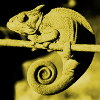
\includegraphics{chamaeleongelb}} + \raisebox{-0.4\height}{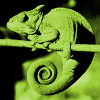
\includegraphics{chamaeleongruen}} $\longrightarrow$ $2 \cdot$ \raisebox{-0.4\height}{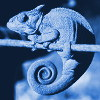
\includegraphics{chamaeleonblau}}
  \quad $\Big\vert$ \quad 
  \raisebox{-0.4\height}{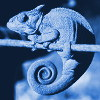
\includegraphics{chamaeleonblau}} + \raisebox{-0.4\height}{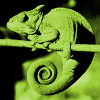
\includegraphics{chamaeleongruen}} $\longrightarrow$ $2 \cdot$ \raisebox{-0.4\height}{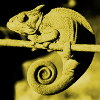
\includegraphics{chamaeleongelb}}
  \quad $\Big\vert$ \quad
  \raisebox{-0.4\height}{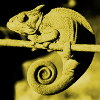
\includegraphics{chamaeleongelb}} + \raisebox{-0.4\height}{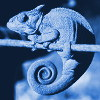
\includegraphics{chamaeleonblau}} $\longrightarrow$ $2 \cdot$ \raisebox{-0.4\height}{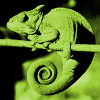
\includegraphics{chamaeleongruen}}
\end{center}

Grundsätzlich könnte diese Situation eintreten, da $345 + 346 + 347 = 1038$ durch $3$ teilbar ist. Wenn wir allerdings versuchen, eine Liste von Begegnungen zu erstellen, sodass nach diesen Begegnungen die Anzahl der Chamäleons jeder Farbe gleich ist, scheitern wir. Spoiler: Auch diese Aufgabe ist nicht lösbar.

Was hat diese Aufgabe nun mit den Schachbrettaufgaben gemeinsam? Zunächst haben wir eine Anfangssituation, beispielsweise das leere (verkleinerte) Schachbrett oder die Anzahlen der Chamäleons auf der Insel. Dann verändert sich die Ausgangslage durch Züge (das Legen eines Dominosteins) oder Ereignisse (Treffen von zwei Chamäleons). Die Frage in beiden Aufgaben ist, ob eine bestimmte Situation (alle Felder bedeckt bzw. gleich viele Chamäleons von jeder Farbe) eintreten kann.

In beiden Aufgabentypen finden wir experimentell keine Lösung und suchen daher nach einem Grund, warum wir jedes solche Unterfangen von vornherein zum Scheitern verurteilt ist. In der Schachbrettaufgabe könnten wir dies begründen, indem wir alle Möglichkeiten ausprobieren. Davon gibt es allerdings ziemlich viele, sodass wir eine Antwort auf diesem Weg - wenn überhaupt - nur mit Hilfe eines Computers finden können. In der zweiten Aufgabe allerdings, gibt es (auf den ersten Blick) unendlich viele Möglichkeiten, wie sich Chamäleons treffen können; wenn wir beispielsweise herausgefunden haben, dass wir mit 40 Treffen von Chamäleons die gewünschte Endsituation nicht erreichen können, so könnte uns das 41 Treffen zum Ziel führen.

Wir haben uns daher in der Aufgabe mit dem Schachbrett eines anderen Tricks bedient: Wir haben bemerkt, dass am Anfang das verkleinerte Brett $32 - 30 = 2$ schwarze Felder mehr besitzt als weiße Felder. Jedes Mal, wenn wir einen Dominostein gelegt haben, wurde ein weißes und ein schwarzes Feld verdeckt, also blieb die Differenz zwischen der Anzahlen der schwarzen offenen und weißen offenen Felder immer gleich. Wir haben also eine Zahl entdeckt, die wir für jedes unbedeckte, teilweise oder vollständig mit Steinen bedeckte Spielbrett ausrechnen können und die mit jedem weiteren platzierten Stein, egal wo er gelegt wird, gleich bleibt. Man sagt auch, dass diese Zahl unverändert (mit Fremdwort invariant) bleibt und nennt sie eine \emph{Invariante}. In der gewünschten Endposition, dass das ganze Brett belegt ist, wäre die Differenz zwischen den offenen schwarzen und offenen weißen Feldern gleich $0 - 0 = 0$. Diese Situation kann also beginnend bei unserer Anfangsposition nicht erreicht werden.

Es ist nicht möglich, dass es irgendwann gleich viele Chamäleons von jeder Farbe gibt. Wir betrachten die Zahl $C$, die wir als Differenz zwischen der Anzahl der blauen und grünen Chamäleons festlegen. Zu Beginn ist
	\[C = \text{Zahl der blauen Chamäleons } - \text{Zahl der grünen Chamäleons } = 347 - 346 = 1.\]
Nun schauen wir, was mit dieser Zahl passiert, wenn sich verschiedene Chamäleons treffen (und dabei ihre Farbe ändern):
\begin{itemize}
	\item Wenn sich ein blaues und ein grünes Chamäleon treffen, so bleibt die Zahl $C$ gleich (denn sowohl die der blauen als auch die der grünen Chamäleons nimmt um eins ab).
	\item Wenn sich allerdings ein grünes und ein gelbes Chamäleon treffen, so nimmt die Zahl der grünen Chamäleons um eins ab, während die Zahl der blauen um zwei steigt. Insgesamt erhöht sich $C$ um drei (wenn dir nicht klar ist, warum, dann spiele diese Situation einfach mal mit konkreten Zahlen durch und beobachte wie sich $C$ dabei verändert).
	\item Wenn sich ein blaues und ein gelbes Chamäleon treffen, so sinkt $C$ um drei (mit ähnlicher Begründung).
\end{itemize}

Die Zahl $C$ ist also nicht invariant. Aber wir stellen fest: Zu Beginn ist $C$ gleich 1, also nicht durch 3 teilbar. Wir wissen aber auch: Wenn eine ganze Zahl $k \in \ZZ$ durch 3 teilbar ist, so sind auch die Zahlen $k + 3$ und $k - 3$ durch 3 teilbar\footnote{Erinnerst du dich noch an den zweiten Korrespondenzbrief? Da haben wir das gezeigt!}. Umgekehrt ist, wenn $k \in \ZZ$ nicht durch 3 teilbar ist, auch die Zahlen $k + 3$ und $k - 3$ nicht durch 3 teilbar. 

Also können wir folgern, dass nach jedem Treffen von zwei Chamäleons unsere Zahl immer noch \emph{nicht} durch 3 teilbar ist. Unsere Invariante ist hier also nicht die Zahl $C$ selbst, sondern die Tatsache, dass $C$ nicht durch 3 teilbar ist. 

In der gewünschten Endsituation wäre $C = 0$, da wir verlangen, dass die Zahl der blauen und grünen Chamäleons dann gleich ist, und $0$ durch $3$ teilbar ist! Folglich kann diese Situation nicht erreicht werden.

\begin{aufgabe}{}
	Mit den nun gesammelten Aufgaben: Kannst du eine Startsituation angeben, aus der heraus es möglich ist gleich viele gelbe, blaue und grüne Chamäleons zu erhalten (gib auch an, wie man das erreichen kann)?
	
	Kannst du außerdem noch eine andere Startsituation angeben, aus der heraus es nicht möglich ist gleich viele Chamäleons jeder Farbe zu erhalten?
\end{aufgabe}

\begin{aufgabe}{Chamäleonmünzen}
	Für dieses Spiel brauchst du sechs Münzen. Lege zwei davon mit der Zahl nach oben vor dich und die restlichen mit dem Bild nach oben. Dein Ziel ist es nun so lange Münzen umzudrehen, bis gleich viele Münzen mit Zahl oben wie Münzen mit Bild oben vor dir liegen. Damit diese Aufgabe nicht zu einfach wird, musst du dabei allerdings immer \emph{genau zwei Münzen auf einmal } umdrehen. Du kannst also pro Spielzug entweder zwei Zahlmünzen zu Bildmünzen machen, zwei Bildmünzen zu zwei Zahlmünzen oder eine Zahl- und eine Bildmünze zu einer Bild und einer Zahlmünze:
	
	\begin{center}
		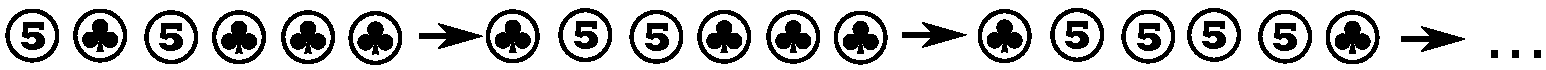
\includegraphics[width=.9\textwidth]{Bilder/Muenzen.pdf}
	\end{center}
	
	Ist es möglich mit dieser Vorgabe das Ziel zu erreichen? Falls ja, gib den Weg dazu an (du kannst dazu zum Beispiel die einzelnen Spielsituationen wie oben gezeigt nacheinander aufmalen). Falls nein, kannst du beweisen, dass es nicht möglich ist das Ziel zu erreichen? 
	
	Wie ist es, wenn wir die Regel ein wenig abändern, sodass du nun immer \emph{genau drei Münzen auf einmal} umdrehen darfst? Ist es jetzt möglich das Ziel zu erreichen?
	
	\emph{Hinweis:} Wenn du beweisen möchtest, dass es nicht möglich ist das Ziel zu erreichen, bietet sich eine Invariante ähnlich zu der in der Chamäleonaufgabe an. Evtl. solltest du aber auf Teilbarkeit durch eine andere Zahl prüfen. Prüfe bei deiner Invariante wieder wie sich diese bei den verschiedenen Spielzügen verändert!
\end{aufgabe}

\begin{aufgabe}{}
	Wir wollen noch einmal das gleiche Spiel spielen, diesmal aber mit acht Münzen. Von diesen zeigen zu Beginn drei Stück eine Zahl und die übrigen fünf Stück ein Bild.
	
	Ist es hier möglich gleich viele Kopfmünzen wie Bildmünzen zu erhalten, wenn du
	\begin{enumerate}
		\item pro Spielzug genau zwei Münzen umdrehen musst?
		\item pro Spielzug genau drei Münzen umdrehen musst?
		\item pro Spielzug genau vier Münzen umdrehen musst?
	\end{enumerate}
\end{aufgabe}


\section{Mehr Invarianten}

Invarianten sind ein nützliches Mittel für Aufgaben obiger Art, bei denen man zeigen soll, dass eine bestimmte Situation nicht erreicht werden kann. Ein Nachteil dieser Technik ist es, dass Invarianten oft nicht offensichtlich sind, sondern es einiger Kreativität und Erfahrung bedarf, um sie zu finden. Bei der Schachbrettaufgabe könnte man feststellen, dass am Ende jedes Versuches zwei schwarze Felder übrig bleiben. Generell bietet sich an, wenn man so eine Aufgabe angeht, erst einmal herumzuprobieren und dabei Zahlen, die einem wichtig erscheinen, nach jedem Schritt aufzuschreiben und danach nach Mustern zu suchen.

Auch in der höheren Mathematik spielen Invarianten eine wichtige Rolle: Es gibt beispielsweise eine Teilgebiet der Mathematik, das sich mit Knoten befasst. Einen Knoten stellt man sich dabei als Seil im dreidimensionalen Raum vor, wobei Anfang und Ende des Seils zusammengebunden sind. Wenn wir einen Knoten haben, so stellen sich Mathematiker die Frage, ob wir diesen Knoten nur durch Bewegen des Seiles (ohne Zerschneiden) auflösen können, sodass er nur noch aus einer einfachen Seilschlinge besteht. Um zu beweisen, dass dies für manche Knoten nicht möglich ist, haben Mathematiker Invarianten gefunden, die etwas komplizierter als unsere bisher gesehene Invarianten sind und beim Umformen eines Knoten gleich bleiben.

Im folgenden findest du nochmal zwei weitere Aufgaben, in denen du selbst versuchen kannst eine passende Invariante zu finden:

\begin{aufgabe}{}
	Wir beginnen mit den Zahlen von $1$ bis $8$, die nebeneinander aufgeschrieben sind:
		\[1 \quad\vert\quad 2 \quad\vert\quad 3 \quad\vert\quad 4 \quad\vert\quad 5 \quad\vert\quad 6 \quad\vert\quad 7 \quad\vert\quad 8\]
	In jedem Spielzug wählst du nun zwei Zahlen aus und bildest Summe und Differenz dieser beiden Zahlen. Dann ersetzt du eine der beiden Zahlen durch die Summe und die andere durch die Differenz. Wählst du zum Beispiel $3$ und $7$, so erhältst du im nächsten Schritt:
		\[1 \quad\vert\quad 2 \quad\vert\quad \mathbf{10} \quad\vert\quad 4 \quad\vert\quad 5 \quad\vert\quad 6 \quad\vert\quad \mathbf{4} \quad\vert\quad 8\]
	(denn $3+7=10$ und $7-3=4$). Wählst du dann $10$ und $4$, so erhältst du
		\[1 \quad\vert\quad 2 \quad\vert\quad \mathbf{6} \quad\vert\quad 4 \quad\vert\quad 5 \quad\vert\quad \mathbf{14} \quad\vert\quad 4 \quad\vert\quad 8\]
	usw.
	
	Dein Ziel ist es nun durch mehrere solche Spielzüge irgendwann in folgende Situation zu kommen:
		\[2 \quad\vert\quad 2 \quad\vert\quad 2 \quad\vert\quad 2 \quad\vert\quad 2 \quad\vert\quad 2 \quad\vert\quad 2 \quad\vert\quad 2\]		
	Ist das möglich? Falls ja, wie? Falls nein, kannst du das beweisen (etwa indem du eine Invariante angibst, die in jedem Spielzug erhalten bleibt)?
	
	\emph{Zusatzaufgabe:} Ist es überhaupt möglich in eine Spielsituation zu kommen, in der nur noch lauter gleiche Zahlen da stehen?
\end{aufgabe}

\begin{aufgabe}{Produkte und Summen auf dem Schachbrett\footnote{Diese Aufgabe basiert auf einer Aufgabe aus dem 4. Landeswettbewerb Mathematik Bayern}}
	Die Felder eines Schachbretts sind in beliebiger Reihenfolge mit den Zahlen $1$ bis $64$ belegt. Du darfst nun zwei Felder auswählen und bildest die Summe und das Produkt ihrer Zahlen. Danach wird die Zahl des einen Feldes durch diese Summe und die Zahl des anderen Feldes durch dieses Produktes ersetzt. 
	
	Kannst du durch mehrfache Anwendung dieses Verfahren erreichen, dass auf allen Feldern die gleiche Zahl steht?
	
	\emph{Hinweis:} Was passiert, wenn du zwei gerade Zahlen auswählst? Was bei zwei ungeraden Zahlen? Bei einer ungeraden und einer geraden Zahl?
\end{aufgabe}

\newpage

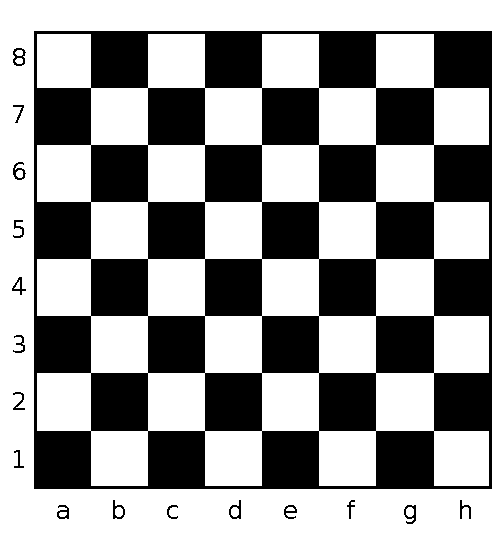
\includegraphics[scale=.8]{Bilder/Schachbrett.pdf}
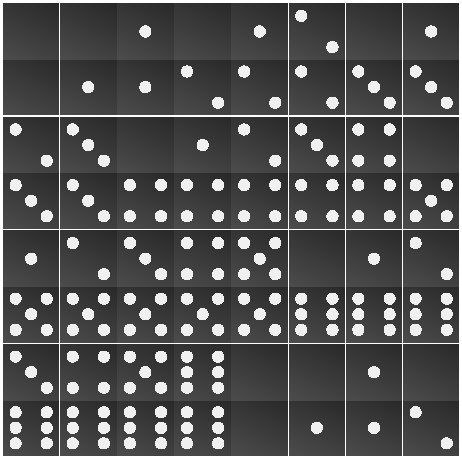
\includegraphics[scale=.8]{Bilder/Dominosteine.pdf}

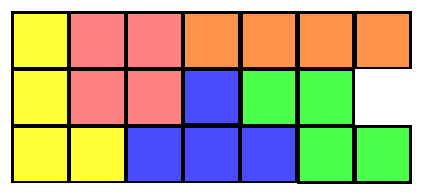
\includegraphics[scale=.8]{Bilder/Tetrominos-kompakt.pdf}
\includegraphics[scale=.4]{Bilder/DreiecksTetrominos-kompakt.pdf}

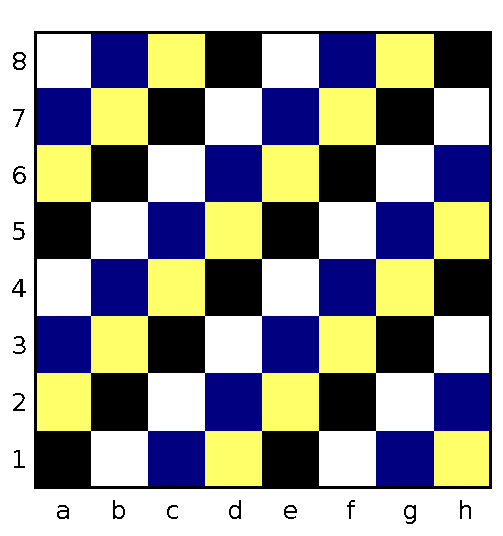
\includegraphics[scale=.8]{Bilder/ViererSchachbrett1.pdf}
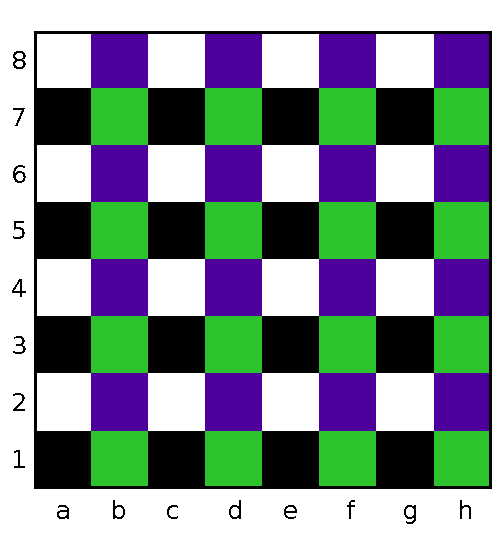
\includegraphics[scale=.8]{Bilder/ViererSchachbrett2.pdf}

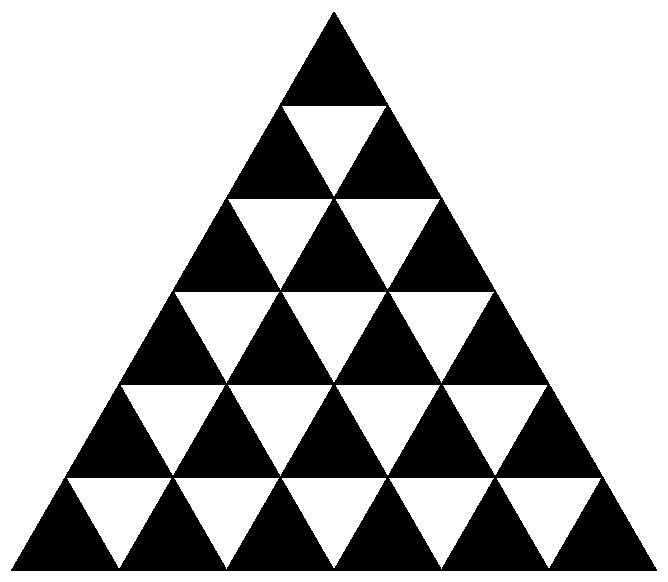
\includegraphics[scale=.4]{Bilder/Dreiecksschachbrett.pdf}
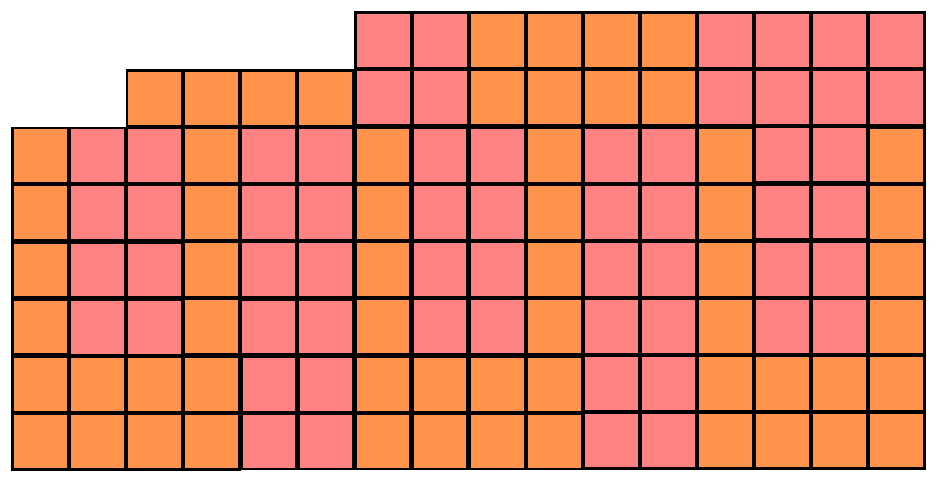
\includegraphics[scale=.8]{Bilder/Tetrominos-extra.pdf}

\end{document}